\documentclass{beamer}
 
\usepackage[utf8]{inputenc}

\usetheme{Madrid}
\usecolortheme{default}

\usepackage[qm]{qcircuit}
\usepackage{bibentry}




\usepackage{tikz,tikz-cd}












\usepackage{physics}
\usepackage{amsmath}
\usepackage{amsfonts}
\usepackage{esint}
\usepackage{bbold}
\usepackage{mathtools}
\usepackage{dsfont}
\usepackage{amsthm}
\usepackage{bbm}
\usepackage{amssymb}
\theoremstyle{definition}
\newtheorem{defn}{Definition}[section]
\newtheorem{prop}{Properties}[section]
\newtheorem{rmk}{Remark}[section]
\newtheorem{exmp}{Example}[section]
\newtheorem{prob}{Problem}[section]
\newtheorem{sln}{Solution}[section]
\newtheorem{thm}{Theorem}[section]
\newtheorem*{prob*}{Problem}
\newtheorem*{sln*}{Solution}
\usepackage{empheq}
\usepackage{tensor}
\usepackage{hyperref}
\usepackage{xcolor}

\newcommand{\R}{\mathbb{R}}
\newcommand{\F}{\mathcal{F}}
\newcommand{\p}{\partial}

\newcommand{\V}{\mathbf{V}}
\newcommand{\W}{\mathbf{W}}
\newcommand{\Z}{\mathbf{Z}}
\newcommand{\Y}{\mathbf{Y}}
\newcommand{\U}{\mathbf{U}}
\newcommand{\X}{\mathbf{X}}

\newcommand{\A}{\mathcal{A}}
\newcommand{\B}{\mathcal{B}}

\newcommand{\xpan}{\text{span}}

\newcommand{\lag}{\mathcal{L}}

\newcommand{\J}{\mathbf{J}}

\newcommand{\M}{\mathcal{M}}

\newcommand{\lp}{\left(}
\newcommand{\rp}{\right)}

\newcommand{\lb}{\left[}
\newcommand{\rb}{\right]}

\newcommand{\lc}{\left\{}
\newcommand{\rc}{\right\}}

\newcommand{\K}{\mathcal{K}}

\newcommand{\N}{\mathcal{N}}

\newcommand{\E}{\mathcal{E}}

\newcommand{\ima}{\text{Im}}
\newcommand{\lin}{\overset{\text{linear}}{\longrightarrow}}
\newcommand{\T}{\mathcal{T}}
\newcommand{\poly}{\mathbb{P}}
\newcommand{\s}{\mathcal{S}}

\newcommand{\gives}{\rotatebox[origin=c]{180}{$\Rsh$}	}


\newcommand{\bigzero}{\mbox{\normalfont\Large\bfseries 0}}
\newcommand{\rvline}{\hspace*{-\arraycolsep}\vline\hspace*{-\arraycolsep}}




 
 
%Information to be included in the title page:
\title{PDE's \& Calculus of Variations}
\author[Huan Q. Bui] % (optional)
{Huan Q. Bui}

\institute[Colby College] % (optional)
{
	
	MA411: PDE
	\and
	Professor Evan Randles
}
\date{May 6, 2019}
 
%\logo{
\includegraphics[height=0.3cm]{colby.png}}
 
\begin{document}
 
\frame{\titlepage}

%%%%%%%%%%%%%%%%%%%%%%%%%%%%%%%%%%%%%%%%%%%%%%%%%%%%%%%%%%%%%%%%%%%%%%%%%



%\begin{frame}[fragile]
%\begin{center}
%	$\,$\Qcircuit @C=.7em @R=.4em  {
%		\lstick{a: \ket{0}} & \qw & \qw & \targ & \meter & \qw \\
%		\lstick{b: \ket{0}} & \qw & \gate{H} & \ctrl{-1}& \meter & \qw 
%	}
%\end{center}
%\end{frame}


%%%%%%%%%%%%%%%%%%%%%%%%%%%%%%%%%%%%%%%%%%%%%%%%%%%%%%%%%%%%%%%%%%%%%%%%%

 
\begin{frame}
\frametitle{Presentation layout}
\tableofcontents
\end{frame}

%%%%%%%%%%%%%%%%%%%%%%%%%%%%%%%%%%%%%%%%%%%%%%%%%%%%%%%%%%%%%%%%%%%%%%%%%

\section{Silly motivating example}

\begin{frame}
\frametitle{Shortest arc joining two points on a plane}
\pause
\underline{Idea}: Let the ``correct'' path be $\bar{y}(x)$, then any path is
\begin{align*}
y(x) = \bar{y}(x) + \epsilon \eta(x)
\end{align*} 
where $\eta(x_1) = \eta(x_2) = 0$, and $\epsilon$ is some constant parameter. 
\pause
\begin{figure}[h!]
	\centering
	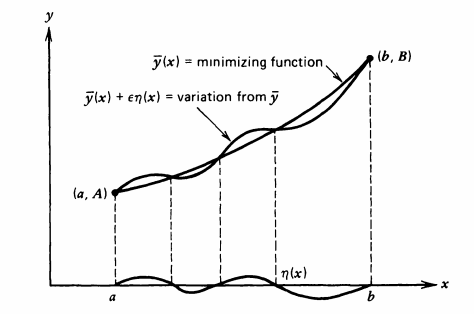
\includegraphics[scale=0.4]{path.png}
\end{figure}
\pause
Distance, for any given variation $\eta(x)$:
\begin{align*}
L(\alpha) = \int\,ds = \int^{x_2}_{x_1}\sqrt{1+(y')^2}\,dx
\end{align*}

\end{frame}

%%%%%%%%%%%%%%%%%%%%%%%%%%%%%%%%%%%%%%%%%%%%%%%%%%%%%%%%%%%%%%%%%%%%%%%%%

\section{The general picture}

\begin{frame}
\frametitle{The general picture...}
\pause
\begin{align*}
S(\epsilon) = \int^{b}_a f[y',y,x]\,dx = \int^b_a f[\bar{y}'+\epsilon\eta',\bar{y}+\epsilon\eta,x]\,dx.
\end{align*}
\pause
\underline{Necessary condition}: if $\bar{y}$ minimizes $S(\epsilon)$, then \pause
\begin{align*}
\frac{\p S}{\p \epsilon} = 0 \implies 0 = \frac{\p f}{\p \epsilon} = \eta \frac{\p f}{\p y} + \eta'\frac{\p f}{\p y'}.
\end{align*}
\pause Can show: \pause
\begin{align*}
\frac{\p S}{\p \epsilon} = \int^b_a \eta(x)\left( \frac{\p f}{\p y} - \frac{d}{dx}\frac{\p f}{\p y'}\right)\,dx = 0.
\end{align*}
\pause This is true for any $\eta(x)$, so \pause 
\begin{align*}
\boxed{\frac{\p f}{\p y} - \frac{d}{dx}\frac{\p f}{\p y'} = 0}
\end{align*}
$\longrightarrow$ \textbf{Euler-Lagrange equation}.
\end{frame}


%%%%%%%%%%%%%%%%%%%%%%%%%%%%%%%%%%%%%%%%%%%%%%%%%%%%%%%%%%%%%%%%%%%%%%%%%


\section{Back to example}


\begin{frame}
\frametitle{Back to silly example}
\pause
\begin{align*}
f[y',y,x] = \sqrt{1 +(y')^2}
\end{align*}
\pause
Applying the Euler-Lagrange equations: \pause
\begin{align*}
&\frac{\p f}{\p y} - \frac{d}{dx}\frac{\p f}{\p y'} = 0\\
\implies& y' = \text{Constant}\\
\implies& y = ax + b.
\end{align*}
$\longrightarrow$ a straight line as expected. 
\end{frame}


%%%%%%%%%%%%%%%%%%%%%%%%%%%%%%%%%%%%%%%%%%%%%%%%%%%%%%%%%%%%%%%%%%%%%%%%%


\section{Why?}
\begin{frame}
\frametitle{A powerful method: Answer isn't always obvious}
\pause
\underline{Ex}: The Brachistochrone problem by Bernoulli, 1696. 
\begin{figure}[h!]
	\centering
	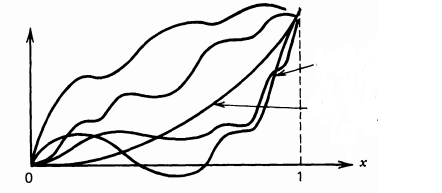
\includegraphics[scale=0.3]{brac.png}
\end{figure} 
\underline{Goal}: minimize sliding time on a frictionless path.
\pause
\begin{align*}
Time = \frac{1}{\sqrt{2g}}\int^{y_2}_{y_1}\sqrt{\frac{1+(x')^2}{y}}\,dy.
\end{align*}
\pause
Applying Euler-Lagrange equation to $f[x',x,y]$, get
\pause
\begin{align*}
\begin{cases}
x = a(\theta - \sin\theta)\\
y = a(1-\cos\theta)
\end{cases} \longrightarrow \text{Cycloid}
\end{align*}
\end{frame}

%%%%%%%%%%%%%%%%%%%%%%%%%%%%%%%%%%%%%%%%%%%%%%%%%%%%%%%%%%%%%%%%%%%%%%%%%

\section{Connection to PDE's}

\begin{frame}
\frametitle{Two-way street}

\begin{enumerate}
	\item PDE's can be formulated as minimization problems
	\pause
	\item Euler-Lagrange Equations as PDE's
\end{enumerate}

\end{frame}


%%%%%%%%%%%%%%%%%%%%%%%%%%%%%%%%%%%%%%%%%%%%%%%%%%%%%%%%%%%%%%%%%%%%%%%%%

\subsection{PDE's as minimization problems}


\begin{frame}
\frametitle{PDE's as minimization problems}
\underline{Ex}: Laplace's equation with Dirichlet BC:
\begin{align*}
(\ast)\begin{cases}
\laplacian u = 0 \hspace{0.5cm} \text{in $\Omega$}\\
u = g \hspace{0.5cm} \text{on $\p \Omega$}
\end{cases}
\end{align*}
\pause
\underline{Claim}: Of all admissible $w$ satisfying $w=g$,
 $u$ solves $(\ast) \iff u$ minimizes
\begin{align*}
S[w] = \frac{1}{2}\int_\Omega \vert \nabla w \vert^2\,dx.  
\end{align*} 
\end{frame}

%%%%%%%%%%%%%%%%%%%%%%%%%%%%%%%%%%%%%%%%%%%%%%%%%%%%%%%%%%%%%%%%%%%%%%%%%

\begin{frame}
\frametitle{Proof $\implies$}
\underline{Show}: $u$ solves $(\ast) \implies $ $S[u] \leq S[w]\, \forall \text{ admissible } w$. 
\pause
\begin{align*}
\text{Observe: }0 = \int w\laplacian u = -\int \nabla u \cdot \nabla w.
\end{align*}
\pause
So,
\begin{align*}
S[u'] = \frac{1}{2}\int\vert\nabla(u+v)\vert^2 = \frac{1}{2}\int \vert\nabla u\vert^2 + \frac{1}{2}\int \vert\nabla w\vert^2 \geq \frac{1}{2}\int \vert\nabla u\vert^2.
\end{align*}
\pause
$\implies $ $u$ minimizes $S[w]$. 
\end{frame}

%%%%%%%%%%%%%%%%%%%%%%%%%%%%%%%%%%%%%%%%%%%%%%%%%%%%%%%%%%%%%%%%%%%%%%%%%

\begin{frame}
\frametitle{Proof $\impliedby$}
\underline{Show}: $u$ minimizes $S[w] \implies $ $u$ solves $(\ast)$.\\$\,$\\
\pause
\underline{Idea}: Consider variation in $u$, so let $u \to u + \epsilon v$, $v$ satisfies BC. 
\pause
\begin{align*}
S[u + \epsilon v] = \frac{1}{2}\int \vert \nabla (u + \epsilon v) \vert^2 = \frac{1}{2}\int \vert \nabla u\vert^2 + 2\epsilon \nabla u\cdot \nabla v + \epsilon^2 \vert \nabla  v \vert^2 .
\end{align*}
\pause
$u$ minimizes $S$, so $\p S/\p\epsilon = 0$ at $\epsilon =0 $, so after a lot of simplification
\begin{align*}
\frac{\p S}{\p \epsilon}\bigg\vert_{\epsilon=0} = -\int v\nabla^2u = 0.
\end{align*}
\pause
This is true for any $v$, so $\boxed{\nabla^2 u = 0}$. So $u$ solves $(\ast)$ as claimed.  
\end{frame}

%%%%%%%%%%%%%%%%%%%%%%%%%%%%%%%%%%%%%%%%%%%%%%%%%%%%%%%%%%%%%%%%%%%%%%%%%

\subsection{Euler-Lagrange Equations as PDE's}
\begin{frame}
\frametitle{Euler-Lagrange Equations as PDE's}
\underline{Recall}: If $y$ minimizes
\begin{align*}
S[y] = \int f[y',y,x]\,dx
\end{align*}
\pause
we have an associated Euler-Lagrange Equation:
\begin{align*}
\frac{\p f}{\p y} = \frac{d}{dx}\frac{\p f}{\p y'}.
\end{align*}
\pause
$\longrightarrow$ Looks complicated, but if $\lag$ is known then things often become simple :)



\end{frame}

%%%%%%%%%%%%%%%%%%%%%%%%%%%%%%%%%%%%%%%%%%%%%%%%%%%%%%%%%%%%%%%%%%%%%%%%%


\begin{frame}
\frametitle{Principle of Least Action}
\begin{align*}
S[y] = \int f[y',y,x]\,dx
\end{align*}
\pause
Associated Euler-Lagrange Equation:
\begin{align*}
\frac{\p f}{\p y} = \frac{d}{dx}\frac{\p f}{\p y'}.
\end{align*}
\pause
In physics, $S$ is called the \textbf{action}. $f$ is called the \textbf{Lagrangian}, denoted $\lag$. \\
\pause
$\,$\\
$\longrightarrow$ \textbf{Principle of Least Action}: Systems tend to be such that $\boxed{\delta S = 0}$\\
\pause
\begin{align*}
\boxed{\lag = \text{Kinetic energy} - \text{Potential Energy}}
\end{align*}
$\longrightarrow$ Equations of motion are found as solutions to E-L PDE's.
\end{frame}


%%%%%%%%%%%%%%%%%%%%%%%%%%%%%%%%%%%%%%%%%%%%%%%%%%%%%%%%%%%%%%%%%%%%%%%%%


\begin{frame}
\frametitle{Newton's Second Law from E-L}
Consider
\pause
\begin{align*}
\lag = \frac{1}{2}mv^2 - U(x) = \lag[x',x,t] = \lag[v,x,t].
\end{align*}
\pause
Then Euler-Lagrange equation tells us
\pause
\begin{align*}
\frac{\p \lag}{\p x} &= \frac{d}{dt}\frac{\p \lag}{\p x'}\\
\onslide<5->{-\frac{d U}{dx} &= \frac{d}{dt}(mv)\\
\onslide<6->{F &= ma}}
\end{align*}
\onslide<7->{$\longrightarrow$ In fact, Laplace's, Poisson's, wave eqns,... can be found this way!}
\end{frame}

%%%%%%%%%%%%%%%%%%%%%%%%%%%%%%%%%%%%%%%%%%%%%%%%%%%%%%%%%%%%%%%%%%%%%%%%%

\begin{frame}
$$\text{THE END}$$
\end{frame}

%%%%%%%%%%%%%%%%%%%%%%%%%%%%%%%%%%%%%%%%%%%%%%%%%%%%%%%%%%%%%%%%%%%%%%%%%


\begin{frame}
\frametitle{Appendix}
\begin{enumerate}
	\item Since $w = 0$ at end points,
	\begin{align*}
	\int w\nabla^2 u = (w\nabla v)\bigg\vert^{b}_a - \int \nabla u\cdot \nabla w =  - \int \nabla u\cdot \nabla w
	\end{align*}

	
	\item \begin{align*}
	\vert \nabla(u+v) \vert^2 = \vert\nabla u\vert^2  + \vert \nabla w\vert^2 + 2\nabla u \cdot \nabla w
	\end{align*}
\end{enumerate}

\end{frame}



\end{document}
